\documentclass[11pt,twoside]{article}
\usepackage{fullpage}
\usepackage{float}
\usepackage{amsmath}
\usepackage{amssymb} 
\usepackage{amsthm}
\usepackage[round]{natbib}
\usepackage{url}
\usepackage{enumerate}
\usepackage{verbatim}
\usepackage{rotating}
\usepackage{booktabs}
\usepackage{longtable}
\usepackage{rotating}
\usepackage{graphicx}
\usepackage{pdflscape}
\usepackage{setspace} 
\usepackage{setspace}

\bibliographystyle{plainnat}

\onehalfspacing

\newtheorem{assumption}{Assumption}
\newtheorem{proposition}{Proposition}


\title{Proposal: The Importance of User Rating of apps: Evidence from apps market of China } 
\author { 
	Tszkin Julian Chan\footnote{Boston University, Department of Economics, 270 Bay State Road, Boston, MA, 02215. E-mail: \protect\url{cjulian@bu.edu}} 
	\and Pucheng Liu \footnote{E-mail:  \protect\url{liupc2008@gmail.com}} 
	\and Yanfei Wang \footnote{ Capital University of Economics and Business. E-mail: \protect\url{yanfei330@gmail.com}} 
}

\begin{document}
\maketitle
\begin{abstract}
\noindent \textbf{JEL Classification: } 

\noindent \textbf{Keywords: Apps Market, Dynamic Panel Model, Instrumental variables, User Review}  

\end{abstract}
\newpage


\section{Objective}
Our objective is to identify the causal effect of the users' rating and the official ranking from the app store on the number of downloads of an mobile app. Our results provide information for apps company to formulate their marketing strategy and pricing information for apps store company (ranking or option to remove negative review)

\section{Model}

\begin{eqnarray} \label{eq:basic_eq}
	downloads_{it} &=& x_{it}^{'} \beta_{x} + Rating_{it}^{'} \beta_{rating} + Ranking_{it}^{'} \beta_{ranking} + \\
	&& \alpha_i + Categories + TimeEffect +  downloads_{it-1} \rho + \varepsilon_{it}
\end{eqnarray}
	
	The variable of interest is the number of downloads and the parameters of interests are $Rating_{it}$ and $Ranking_{it}$ for app $i$ during period $t$. 

\begin{itemize}
	\item $downloads_{it}$ is the number of downloads for app $i$ during period $t$.
	\item $Rating_{it}$ are measurement of the user rating for app $i$ at period $t$. For example, it could be the proportion of positive rating in the different pages(one variable for one page). We might also include the product of positive rating and negative rating, which would capture the variance of the user rating \footnote{Variance of bernoulli distribution is $p(1-p)$}. 
	\item $Ranking_{it}$ are measurement of the ranking or position of the app, which are computed by the apps store company using unknown algorithm(May be we could have some information about this?). 
	\item $x_{it}$ are time varying characteristics of the app. For example, the number of visitor to the web page(or visit with wandoujia's app) of app $i$. The visitor count have potential to become an important variables. It could be a measurement of the strength of advertisement. It is also highly related to the ranking variables. If the ranking of the app is higher, then the visitor count should also be higher, but not necessary the downloads. 
	\item $\alpha_i$ is the app fixed effect. We may also include version fixed effect.
	\item $Categories$ are variables to capture the categories fixed effect. In fact, it should be an interaction terms to other variables. An alternate way is to model the above equation by categories, but it require each apps belong to only one category.
	\item $TimeEffect$ capture possible time trend, seasonality and holiday effect. 
	\item $y_{it-1}$ captures possible autocorrelation of the downloads. 
\end{itemize}

\subsection{Others information}
	Besides the information the user can observe, the following information could be valuable in this study
\begin{itemize}
	\item User data. When a user downloads an app, do we know what other apps do this user have? When do they install them? Since the user has to install an app from wandoujia, this information may be available. With this information, we may be able to estimate relationship across different apps. For example, WeChat and Whatapps should be substitutes, but camera apps and photo editing apps should be complements. With this information, we can further study the user rating dynamic across apps. (For example, if there are a lot of negative rating in Whatapps, would it boost the downloads of WeChat?). Although, we can infer the correlation with machine learning methodology(time series correlation of the number of downloads), it's better to have data.   
	\item Number of visitors. In addition to the number of downloads, number of visitor tell us how many people did visit the page but didn't download the apps. Two apps with similar number of downloads but one with much larger number of visitors do tell us something. 
\end{itemize} 

\subsection{Identification}
	To identify the model we have to properly settle the endogenity of the measurement rating. One possible source of endogenity is the downloads and user rating is driven by the same apps characteristics. For example, if the apps is good, then it should have high number of downloads and a lot of positive rating. However, this correlation does not identify the  causal relationship of number of downloads and user rating. This type of endogenity is captured by the apps(or version) fixed effect $\alpha_i$. To remove the product fixed effect, we can take first difference to equation (\ref{eq:basic_eq})
	
\begin{eqnarray} \label{eq:diff_equation}
	\Delta downloads_{it} &=& \Delta x_{it}^{'} \beta_{x} + \Delta Rating_{it}^{'} \beta_{rating} + \Delta Ranking_{it}^{'} \beta_{ranking} + \\
	&& \Delta TimeEffect +  \Delta downloads_{it-1} \rho + \Delta \varepsilon_{it}
\end{eqnarray}
	
	After removed the fixed effect, $\Delta downloads_{it-1}$ is correlated with $\Delta \varepsilon_{it}$ but we can use the lagged value of  $\Delta downloads_{it-1}$ as instruments to $\Delta downloads_{it-1}$. This is the standard strategy proposed by ArellanoBond(1991) and Holtz-EakinNeweyRosen(1988). 
	
	
	Another possibility is reverse causality. Some of the measurements of user rating could be affected by the number of downloads. For example, total number of user rating or the how frequency of the user rating would depend on the number of downloads. However, the lagged value of rating may not directly affect the number of downloads. If only a few new entries of rating, then the rating measurement should be highly correlated overtime. Therefore, the lagged value of rating could be an instruments. 
	
	We could apply similar argument to the ranking variables. 
	
	To sum up, we can estimate equation (\ref{eq:diff_equation}) using GMM with instruments $\Delta x_{it}$, $\Delta Rating_{it-s} $, $\Delta Ranking_{it-s}^{'} $, $ \Delta downloads_{it-s}$ for $s\geq 2$.
	Intuitively, our identification strategy is to make use of the information in the short term variation of the previous value rating, ranking and downloads. These variables should be uncorrelated with the apps fixed effect and the current shock to the downloads.
	
\subsection{Additional Strategy: Release date of a new version}
The release date of a new version of an apps may help us to identify the model. Assume the user do not know the release date of a new version of the apps(or they didn't care). We can separate the information from the rating variables into two parts, rating before and after the new version. Notice that the rating information before the new version shouldn't contain any information about the quality of current version (after controlling for for apps fixed effect). On the other hand, it affects the rating the user could observe. Therefore, the rating information before the new version could be an instrument for the rating information which the user observed. 

\subsection{Hidden algorithm from the company(wandoujia)}
If we have some information about how the company(wandoujia) rank those apps, it may help us to identify the model. For example, if the company modify the ranking algorithm of the apps, we could have a perfect instrument. 

\subsection{Extensions}
\begin{itemize}
\item The effects of one app's ratings (downloads) on competitive apps (and complementary apps)

\item The effects of ratings (downloads) on developers' decision to update this app
\end{itemize}

\section{Data Structure}
We could store the raw data in the format of a relational data. The data contains 3 data tables, apps, counts and rating. Each row of the data tables is a record, each column is a field/attribute. The data structure will be described by the following ERD (Entity Relationship Diagram) 

\begin{center}
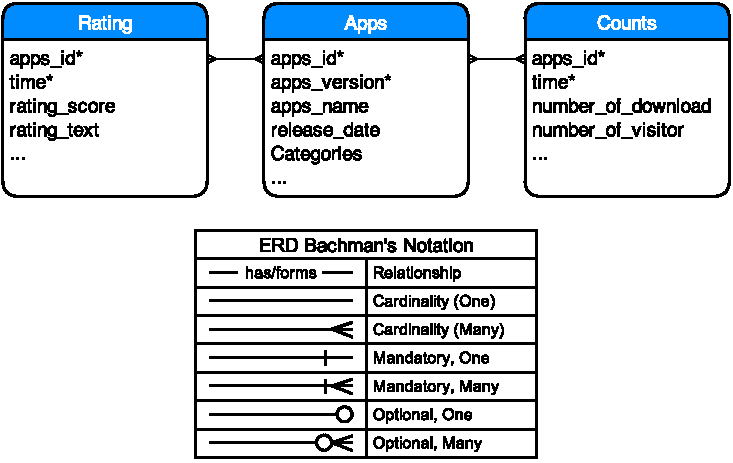
\includegraphics{erd1.pdf}
\end{center}

\subsubsection*{Remark}
\begin{itemize}
	\item * represents primary id. 
	\item ... represents other relevant variables.
	\item The sampling frequency preferred to be less than or equal to a day. (may be 6 or 12hrs)
	\item Categories could be more than one variables
\end{itemize}


\section{Literature}
\newpage

\bibliography{refs}
\bibliographystyle{chicagomod0.0.3d}

\newpage

\appendix
\renewcommand{\thesection}{Appendix \Roman{section}}
\renewcommand{\thesubsection}{Appendix \Roman{section}(\roman{subsection})}


\end{document}
